\section{Техническое задание}
\subsection{Основание для разработки}

Основанием для разработки является задание на выпускную квалификационную работу бакалавра "<Программная система для разработки приключенческих игр">.

\subsection{Цель и назначение разработки}

Основной задачей выпускной квалификационной работы является разработка программной системы приключенческих игр для продвижения их популярности. Данный программный продукт предназначен для демонстрации практических навыков, полученных в течение обучения.

Целью данной разработки является создание программной системы для разработки приключенческих игр и популяризация этого игрового жанра.

Задачами данной разработки являются:
\begin{itemize}
\item проектирование интерфейса;
\item разработка архитектуры приложения;
\item проектирование игрового сценария;
\item реализация взаимодействия приложения с пользователем;
\item реализация графики приложения;
\item реализация сохранений действий персонажа;
\end{itemize}

\subsection{Требования пользователя к движку}

Движок должен включать в себя:
\begin{itemize}
    \item загрузку локаций;
    \item загрузку диалогов;
    \item загрузку объектов в их актуальном состоянии;
    \item изменение и сохранение состояний игровых объектов;
    \item изменение состояний локаций;
    \item возможность изменения сюжета игры;
    \item сохранение действий персонажа и общего игрового прогресса;
    \item возможность смены изображений игровых объектов;
    \item возможность изменения игрового сценария.
\end{itemize}

Композиция шаблона игры, созданной на движке, представлена на рисунке ~\ref{maket:image}.

\begin{figure}[ht]
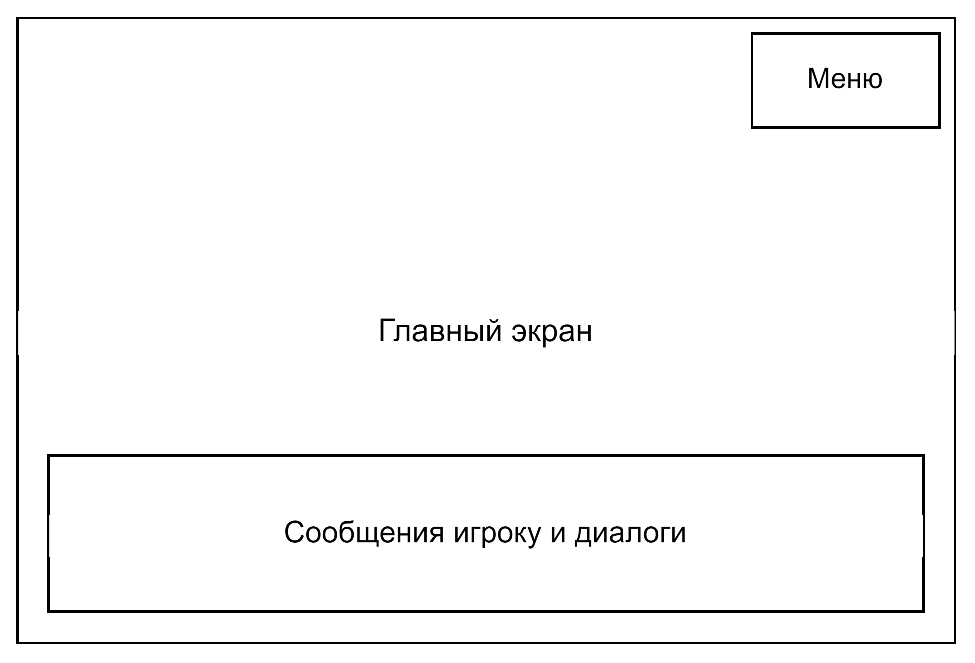
\includegraphics[width=1\linewidth]{maket}
\caption{Композиция шаблона интерфейса игры}
\label{maket:image}
\end{figure}
%\vspace{-\figureaboveskip} % двойной отступ не нужен (можно использовать, если раздел заканчивается картинкой)

\subsection{Правила игры}

В мире, где каждая деталь имеет значение, главный герой (ГГ) отправляется в путешествие, полное тайн и загадок. Игра начинается с захватывающей предыстории, представленной в виде текста на диалоговой панели, который знакомит игрока с основной сюжетной линией и мотивацией ГГ. После вступления ГГ начинает своё приключение, исследуя различные локации и их подлокации, каждая из которых обладает уникальными особенностями и задачами.

Для успешного прохождения игры ГГ должен выполнить ряд квестов, раскрывающихся перед ним по мере продвижения по сюжету. Некоторые локации изначально скрыты и становятся доступными только после выполнения определённых заданий, создавая цепочку событий, которая требует от игрока внимательности и стратегического мышления.

Процесс выполнения квестов включает в себя поиск ключевых предметов, взаимодействие с персонажами и решение головоломок, что позволяет ГГ двигаться вперёд по сюжету. Прогресс игры отслеживается как в целом, так и для каждого квеста в отдельности, позволяя игроку видеть свои достижения.

Интерактивность с миром игры осуществляется через интуитивно понятный интерфейс point-and-click, где каждый объект взаимодействия имеет свои уникальные характеристики:

\begin{enumerate}
	\item \textbf{Дверь} – курсор превращается в миниатюрное изображение двери при наведении, сигнализируя о возможности перехода в новую локацию при выполнении определённых условий.
	\item \textbf{Сущность} – изменение курсора указывает на возможность диалога с персонажем, раскрывающего новые аспекты сюжета или задания.
	\item \textbf{Предмет} – курсор превращается в руку, позволяя игроку подобрать предмет, который затем добавляется в инвентарь, если это допустимо в текущем контексте.
	\item \textbf{Линия} – воображаемая граница, которая может перенести ГГ в другую локацию или остановить его движение, если путь в данном направлении недоступен.
\end{enumerate}

Хотя прямого взаимодействия с инвентарём нет, он играет ключевую роль в прогрессе игры. Если ГГ пытается взаимодействовать с объектом, требующим определённого предмета, который отсутствует в инвентаре, игрок получает соответствующее уведомление. В противном случае, успешное взаимодействие позволяет ГГ продвинуться дальше по сюжету.

Кульминацией игры является финальный квест, после выполнения которого и исследования всех локаций игроку предстоит увидеть развязку истории, ставшую финалом его приключения.

\subsection{Сюжет игры} %ПЕРЕДЕЛАТЬ

В таинственном и манящем лесу, где каждый шорох и каждый луч света кажется чем-то волшебным, маленькая девочка по имени Лилия начинает своё приключение. Она погружается в мир снов, где реальность смешивается с фантазией, и каждый шаг может привести к неожиданным открытиям. Лилия обнаруживает себя в сердце загадочного леса, места, наполненного тайнами и странными существами, которые кажутся знакомыми, но в то же время невероятно далёкими.

С первых же мгновений в этом мире, Лилия сталкивается с обитателем леса, чьё присутствие вызывает у неё смешанные чувства — от любопытства до тревоги. Её первая мысль — покинуть этот сон как можно скорее, но все попытки оказываются тщетными. Осознав, что простое желание проснуться не помогает, она решает исследовать лес в поисках ответов.

Каждая встреча с обитателями леса становится для Лилии новым испытанием и шагом к пониманию этого мира. Они поручают ей задания, которые кажутся простыми на первый взгляд, но каждое из них несёт в себе часть большой загадки. С каждым выполненным квестом Лилия получает не только ключевые предметы или информацию, но и учится видеть мир по-новому, раскрывая его секреты и узнавая о себе что-то важное.

Путешествие приводит её к владыке леса, могущественному и загадочному существу, которое, как говорят, обладает ключом к возвращению в реальный мир. После напряжённого и полного откровений диалога, владыка леса делает нечто неожиданное — он лишает Лилию жизни во сне, что становится катализатором её пробуждения. Сердце девочки замирает на мгновение, и в следующий момент она открывает глаза, лежа в своей кровати, где каждый предмет кажется более ярким, а воздух — свежее, чем когда-либо.


\subsection{Эпизод 1: Лес}

Оказываемся в сумеречном лесу и осматриваемся. На дереве замечаем венок из цветов, при нажатии на него видим сообщение о том, что лучше его не трогать. Неподалеку видим призрака, подходим к нему и нажимаем для взаимодействия. Девочка подмечает: призрак достаточно милый и не страшный. Начинается диалог с призраком, по окончанию которого призрак пытается напугать героиню и строит страшную гримасу. Девочку это не пугает, она лишь смеется над ним и убеждается в том, что находится не в кошмаре. Призрак, услышав насмешливый он девочки моментально увеличивается в размерах и принимает действительно ужасающий вид. Девочка пугается и убегает на другую локацию внутри леса - кладбище. После неудачных попыток проснуться она понимает, что у нее не получается выйти из сна и не известно, что еще ее здесь ждет. На кладбище видим статую плачущего ангела. Когда подходим к ней, слышим звуки плача. Нажимаем на статую и в ходе диалога выясняется, что ветер унес у нее венок с головы и она не может его найти, тк обездвижена. Взамен на эту вещь статуя обещает помочь выбраться из сна. Не найдя эту вещь в данной части леса, движемся в единственную доступную - начальную, где мы встретили призрака. Вспоминаем, что недавно виделись на дереве венок. Увидев призрака, девочка опять испугалась, но не убежала. При осмотре этой локации понимаем, что нужного нам предмета здесь нет, однако достаточно большую часть карты занимает огромный призрак, которого нужно как-то прогнать или уменьшить. Ведь он закрывает собой венок. Девочка не придумала ничего лучше, как напугать его в ответ. Кликаем по ней и смотрим, как она увеличивается в размерах и меняется в лице. Тем временем, по мере увеличения девочки, призрак уменьшается и в конце концов приходит в прежнюю не страшную, а вскоре и совсем убегает. Замечаем, что он закрывал собой тот самый предмет, который мы искали. Забираем его и приносим статуе. Та нас благодарит и говорит, что единственный, кто может помочь ей выбраться из сна - правитель этих земель, а дорогу к нему знает только лис, который спит в этом лесу. Нам открывается путь на следующую локацию этого леса - логово лиса. Зайдя на нее видим большую морду спящего животного. Для того чтобы его разбудить, нужно 3 раза нажать на него. Лис соглашается помочь девочке и провести ее к правителю, но взамен он просит помочь ему с его проблемой: в него что-то залезло и постоянно мешает жить. Лис предлагает девочке залезть к нему в пасть и посмотреть, что там. Нажимаем на пасть лиса и оказываемся в новой локации. Основные объекты и способы  взаимодействия с ними (при нажатии):
\begin{enumerate}
	\item Призрак - говорить.
	\item Статуя - говорить (получить квест), отдать предмет.
	\item Венок – взять, отдать статуе.
	\item Главный герой - вырасти и напугать призрака.
	\item Переход на другую локацию – перейти к призраку, статуе, лису или в пасть к лису.
	\item Лис - разбудить, говорить.
\end{enumerate}

\subsection{Интерфейс пользователя}

На основании анализа предметной области в программе должны быть реализованы следующие прецеденты:
\begin{enumerate}
\item Перемещение по локациям;
\item Перемещение персонажа по игровой области;
\item Просмотр кат-сцен;
\item Просмотр диалогов;
\item Взаимодействие с игровыми объектами при помощи компьютерной мыши.
\end{enumerate}
Таким образом, на рисунке ~\ref{prec:image}сформированы следующие действия пользователя и их последствия.
\begin{figure}[ht]
	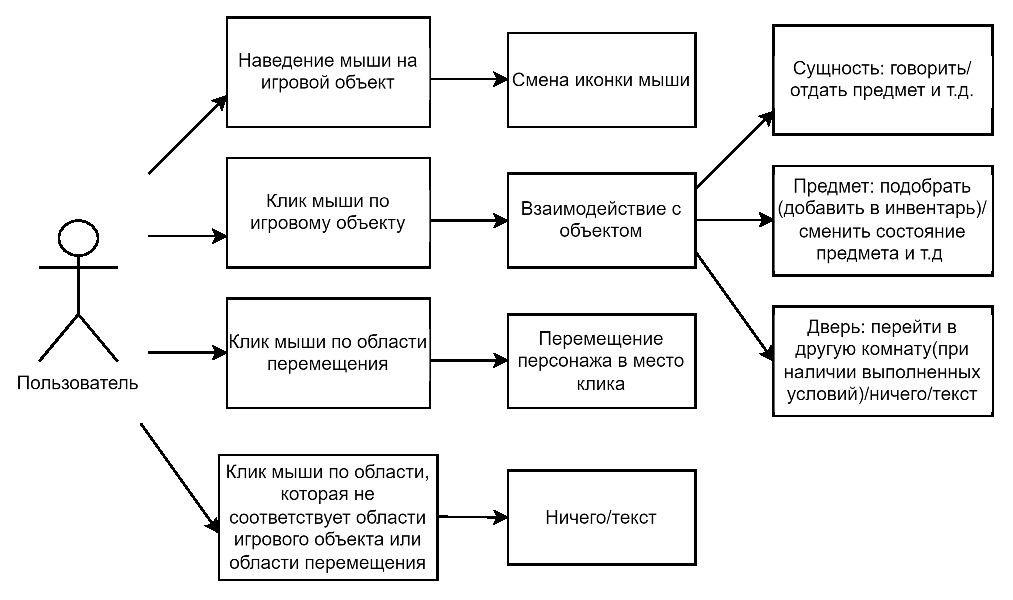
\includegraphics[width=1\linewidth]{prec}
	\caption{Шаблон интерфейса игры}
	\label{prec:image}
\end{figure}
%\vspace{-\figureaboveskip} % двойной отступ не нужен (можно использовать, если раздел заканчивается картинкой)

\subsection{Требования к оформлению документации}

Разработка программной документации и программного изделия должна производиться согласно ГОСТ 19.102-77 и ГОСТ 34.601-90. Единая система программной документации.
